
\section{Definition of compensators}

\begin{frame}
	\frametitle{Lead Compensator vs Lag Compensator}
	\begin{block}{Schematical representation}
		\begin{figure}
			\centering
			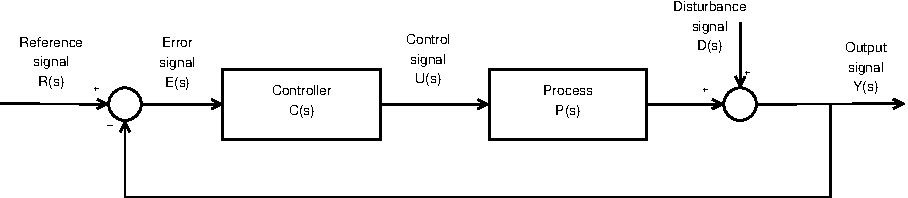
\includegraphics[width=1\linewidth]{Closed-Loop}
		\end{figure}
	\end{block}
	\begin{block}{Transfer functions}
		Lead compensator : 
		$C(s) = K.\frac{s + \frac{1}{\tau}}{s + \frac{1}{\alpha\tau}}$ with $0 \textless  \alpha  \textless  1$ \\
		Lag compensator : 
		$C(s) = K.\frac{s + \frac{1}{\tau}}{s + \frac{1}{\beta\tau}}$ with $\beta  \textgreater  1$
	\end{block}
\end{frame}

\begin{frame}
\frametitle{Lead Compensator vs Lag Compensator: zeros and poles}
\begin{block}{Transfer functions}
	Lead compensator : 
	$C(s) = K.\frac{s + \frac{1}{\tau}}{s + \frac{1}{\alpha\tau}}$ with $0 \textless  \alpha  \textless  1$ \\
	Lag compensator : 
	$C(s) = K.\frac{s + \frac{1}{\tau}}{s + \frac{1}{\beta\tau}}$ with $\beta  \textgreater  1$
\end{block}
\begin{block}{Zeros and poles}
	Zeros: $s = -\frac{1}{\tau}$ \\
	Poles: $s = -\frac{1}{\alpha\tau}$ or $s = -\frac{1}{\beta\tau}$ \\
	For lead compensators the pole lies more to the left in the complex plane than the zero and vice versa for lag compensators.
\end{block}
\end{frame}

\section{Lead compensators}

\begin{frame}
	\frametitle{Lead compensators}
	\begin{block}{Impact}
		$C(s) = K.\frac{s + \frac{1}{\tau}}{s + \frac{1}{\alpha\tau}}$ with $0 \textless  \alpha  \textless  1$
		\begin{figure}
			\centering
			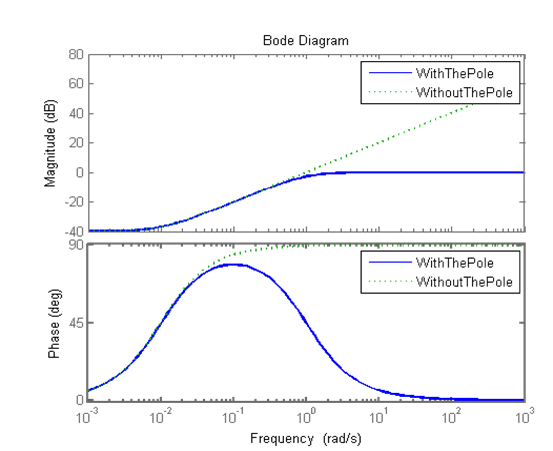
\includegraphics[width=0.5
			\linewidth]{leadcompensator1}
		\end{figure}
	\end{block}
\end{frame}

\begin{frame}
\frametitle{Lead compensators}
\begin{block}{Impact}
	\begin{itemize}
	\item They push the pole of the closed loop system to the left.
	\begin{itemize}
	\item Stabilisation of the system (see root locus)
	\item Increase response speed (lead compensator will stimulate some larger frequencies)
	\end{itemize}
	\item Increase of the phase margin: the phase of the lead compensator is positive for every frequency, and will hence only increase the phase.
	\item Thanks to the presence of a pole, the high frequencies (where most of the unwanted noise is located) are less amplified.
	
	\end{itemize}
\end{block}
\end{frame}

\begin{frame}
\frametitle{Lead compensators}
\begin{block}{Design with Bode plots}
	\begin{itemize}
		\item Design process: tuning of the phase margin, with as a surplus (because we will have one extra degree of freedom) the tuning of the steady state error.
		\item Compensate for the excessive phase lag that is a result of the components of P(s).
		\item Increase in phase at gain crossover frequency (GCF) if GCF is around pole and zero of the lead compensator.
		\item Gain is impacted by the lead compensator: the GCF of P(s).C(s) is not equal to the GCF of P(s).
	\end{itemize}		
\end{block}
\end{frame}

\begin{frame}
	\frametitle{Lead compensators}
	\begin{block}{Design}
		\begin{itemize}
			\item Required increase in phase gain: $\phi$
			\item To compensate for increase GCF due to 
			$C(s) \Rightarrow \phi_m = \phi + 5\,^{\circ}$. This will be needed to determinate $\alpha$ and $\tau$
			\item K will be used to tune the steady state error.
		\end{itemize}		
	\end{block}
\end{frame}
\begin{frame}	
	\frametitle{Lead compensators}
	\begin{block}{Determination of $\alpha$}
		Use polar plot of 
		$\frac{\alpha.(j\omega\tau + 1)}{j\omega\alpha\tau + 1}$	
		\begin{figure}
			\centering
			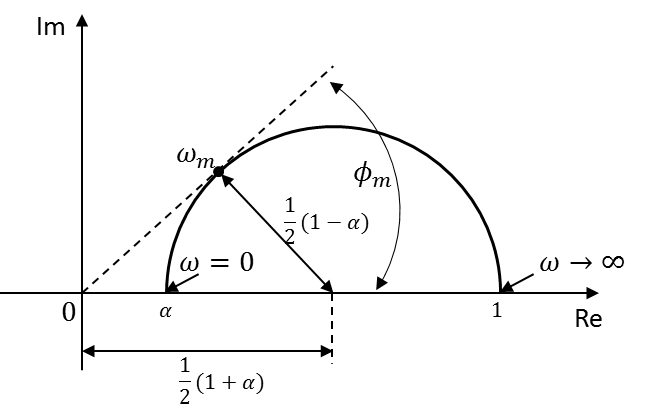
\includegraphics[width=0.5
			\linewidth]{leadcompalphabepalen}
		\end{figure}
		$\sin\phi_m = \frac{\frac{1}{2}.(1 - \alpha)}{\frac{1}{2}.(1 + \alpha)} = \frac{1 - \alpha}{1 + \alpha} \Rightarrow \alpha = \frac{1 - \sin\phi_m}{1 + \sin\phi_m}$ \\
		This relation relates the maximum phase-lead angle and the value of $\alpha$.
	\end{block}
\end{frame}

\begin{frame}
\frametitle{Lead compensators}
\begin{block}{Determination of $\tau$}
	Tekening bodeplot zoals boek p 622.
	The tangent point $\omega_m$ is the geometric mean of the two corner frequencies, so
	$ \log \omega_m = \frac{1}{2}(\log \frac{1}{\tau} + \log \frac{1}{\alpha\tau})$ with $\tau = \frac{1}{\omega}$
	\\ $\Rightarrow \omega_m = \frac{1}{\sqrt{\alpha}\tau}$. \\
	The lead compensator is a high pass filter.
\end{block}
\end{frame}

\begin{frame}
\frametitle{Lead compensators}
\begin{block}{Determination of the tangent point}
	Use the gain crossover frequency of P(s)C(s) as $\omega_m$: \\
	$\mid P(j\omega_m)C(j\omega_m) \mid = 1$ \\
	$\mid P(j\omega_m) \mid K \frac{\sqrt{\frac{1}{\alpha\tau^2} + \frac{1}{\tau^2}}}{\sqrt{\frac{1}{\alpha\tau^2} + \frac{1}{\alpha^2\tau^2}}} = \mid P(j\omega_m) \mid K \sqrt{\alpha} = 1$ \\
	$20\log \mid P(j\omega_m) \mid = -20\log (K\sqrt{\alpha})$ \\
	The value of the tangent point $\omega_m$ can be determined from P(s)'s Bode plot, if you know K (the last freedom).
\end{block}
\end{frame}	

\begin{frame}
\frametitle{Lead compensators}
\begin{block}{Determination of K}
	\begin{itemize}
		\item Remember the steady state error for references of the shape: $\frac{At^n\epsilon(\tau)}{n!}$ with $\epsilon(t)$ the step function.
		\item We found the error constants $K_p$, $K_v$ and $K_a$ as measures for the steady state error for a proportional (n=0), linear (n=1) and accelerating (n=2) reference.
		\item So these error constants can be used to find proper values of K: 
		$\lim_{s \to 0} K \frac{s + \frac{1}{\tau}}{s + \frac{1}{\alpha\tau}}s^nP(s) = K\alpha \lim_{s \to 0}s^nP(s)$
	\end{itemize}
\end{block}
\end{frame}

\begin{frame}
	\frametitle{Lead Compensation Techniques Based on the Frequency-Response Approach}
	\begin{block}{Step 1}
	Find $K\alpha$ from your steady-state requirement.
	\end{block}
	\begin{block}{Step 2}
	Determine $\phi$, the amount with which you want to increase the PM; if the PM is OK, you don’t need a lead compensator; a proportional controller with gain $K\alpha$ suffices.
	\end{block}
	\begin{block}{Step 3}
	Add $5\,^{\circ}$, to get $\phi_m = \phi + 5\,^{\circ}$ (if $\phi_m > 5\,^{\circ}$, you will need more than one lead compensator). The addition of the lead compensator shifts the gain crossover frequency to the right and decreases the
	phase margin.
	\end{block}
\end{frame}

\begin{frame}
	\frametitle{Lead Compensation Techniques Based on the Frequency-Response Approach}
	\begin{block}{Step 4}
	You’ll find $\alpha$ from this $\phi_m$: $\alpha = \frac{1 - \sin \phi_m}{1 + \sin \phi_m}$ and hence also K (see step 1). 
	\end{block}
	\begin{block}{Step 5}
		Find the desired $\omega_m$ by looking at the Bode plot of P(s) and finding the frequency at which the gain equals $-20 \log (K\sqrt{\alpha})$ dB.
	\end{block}
	\begin{block}{Step 6}
	Find $\tau$ as $\frac{1}{\sqrt{\alpha}\omega_m}$.
	\end{block}
\end{frame}

\begin{frame}
	\frametitle{Lead Compensation Techniques Based on the Frequency-Response Approach}
	\begin{block}{Step 7}
		Verify if the system works as asked.
		Check the gain margin to be sure it is satisfactory. If not, repeat the design process
		by modifying the pole-zero location of the compensator until a satisfactory result
		is obtained.
	\end{block}
	\begin{block}{Example}
	Given the system $P(s) = \frac{4}{s(s+2)}$. We want a phase margin of at least $50\,^{\circ}$ and a steady state error for slope reference of maximal $\frac{A}{20}$.
	\end{block}
\end{frame}

\begin{frame}
\frametitle{Example: Bode plot and phase diagram}
Maken in MATLAB.
\end{frame}

\begin{frame}
\frametitle{Example}
\begin{block}{Step 1}
Steady-state requirement: $K_v = \frac{20}{s}$ \\
So, $\lim_{s \to 0} sP(s)C(s) = \lim_{s \to 0} s\frac{s}{s(s+2)}K\alpha = 2K\alpha = 20$. \\
$\Rightarrow K\alpha = 10$
\end{block}
\begin{block}{Step 2}
Phase margin of $K\alphaP(s) = 18\,^{\circ}$ (see phase diagram) \\
$\Rightarrow \phi = 32\,^{\circ}$
\end{block}
\begin{block}{Step 3}
$\phi_m = \phi + 5\,^{\circ} = 37\,^{\circ}$
\end{block}
\end{frame}

\begin{frame}
	\frametitle{Example}
	\begin{block}{Step 4}
	 $\alpha = \frac{1 - \sin \phi_m}{1 + \sin \phi_m} = 0.24$ \\
	 From step 1, we know that $K = \frac{\alpha}{10} = 42$
	\end{block}
	\begin{block}{Step 5}
	Find $\omega_m$, the frequency at which the gain is $-20\log(K\sqrt{\alpha})$ dB. 
	$GCF(P(s)K\sqrt{\alpha}) = GCF(P(s)C(s)) \Rightarrow \omega_m = 9 \frac{rad}{s}$ \\
	(see Bode diagram next slide)
	\end{block}
	\begin{block}{Step 6}
	$\tau = \frac{1}{\omega_m\sqrt{\alpha}} = 0.23$
	\end{block}
\end{frame}

\begin{frame}
	\frametitle{Example}
	\begin{block}{Step 7}
	Verify! MATLAB!!!!
	\end{block}
\end{frame}

\begin{frame}
\frametitle{Summary lead compensators}
\begin{block}{Evaluation of impact}
\begin{itemize}
	\item Pushing the poles to the left: this is not directly visible here, but is linked to the increased band width.
	\item The increase in bandwidth (this is linked to the response speed) and the increase in the phase margin were apparent in the Bode plot of P(s)C(s).
	\item A (small) decrease in the steady-state error occurs, since we designed it as such. \\
	Why small? The steady-state error decreases when the DC gain gets larger, but a lead compensator’s impact on the gain is not really built to increase the DC gain, the shape of a lag compensator is much more fit for this.
\end{itemize}
\end{block}
\end{frame}

\begin{frame}
	\frametitle{Summary lead compensators}
	\begin{block}{Design with root locus}
	Design lead compensators with root locus for time-domain quantities  - use dominant pole locations to fulfill overshoot, rise time, settling time, damping ratio, … requirements.
	\end{block}
\end{frame}

\section{Lag compensators}

\begin{frame}
\frametitle{Lag compensators}
\begin{block}{Impact of lag compensators: Bode diagram}
	MATLAB
\end{block}
\end{frame}

\begin{frame}
	\frametitle{Lag compensators}
	\begin{block}{Transfer function}
		$C(s) = K.\frac{s + \frac{1}{\tau}}{s + \frac{1}{\beta\tau}}$ with $\beta  \textgreater  1$
	\end{block}
	\begin{block}{Impact of lag compensators: Bode diagram}
	\begin{itemize}
		\item Lead compensators: increase the stability and tune the steady-state error by increasing the phase at the crossover frequency.
		\item Impact lag compensator = lead compensator, but different approach!
		By decreasing the gain, the gain crossover frequency comes down to a frequency at which the corresponding phase is higher.
		
	\end{itemize}
	\end{block}
\end{frame}


